\chapter{REFERENCIAL TEÓRICO}

\section{Manufatura Aditiva}
O princípio fundamental da manufatura aditiva (MA) consiste em fabricar um modelo tridimensional de forma 
integrada, dispensando a necessidade de planejar as operações de maneira individual e priorizando a 
consideração das configurações globais.
O processo é calculado pelo fatiador com base em um modelo tridimensional digital,
geralmente criado a partir de \textit{Computer Aided Design} (CAD) e nas configurações do mesmo
e resulta nas intruções necessárias para a máquina de manufatura aditiva construir o modelo físico.
Uma das características 
principais da MA é a rapidez na qual é possível criar protótipo
diretamente de modelos digitais, por conta disso, em um contexto 
de desenvolvimento de produto, o termo prototipagem rápida era 
utilizado. Entretanto, conforme a MA foi se aperfeiçoando era 
perceptível a capacidade dessas tecnologias não só se aterem à 
produção de protótipos, mas também de peças utilizadas em 
produtos finais. Além disso, o termo prototipagem rápida não considerava o princípio 
básico que unia essas tecnologias e assim o termo manufatura 
aditiva foi apresentado e adotado pela \textit{American Society for 
Testing and Materials} (ASTM) \cite{gibson15}.

Atualmente, existe uma grande variedade de tecnologias e processos de manufatura aditiva.
Os métodos de impressão 3D variam na maneira como depositam o material, como extrusão, sinterização a 
laser e estereolitografia. Eles também diferem nos princípios físicos que utilizam, como fusão, cura por luz
e aglutinação. Além disso, os materiais que podem ser utilizados incluem plásticos, resinas, metais e cerâmicas. 
Como mencionado anteriormente, um dos métodos de manufatura aditiva mais populares
é a tecnologia FDM, entretanto existem diversas outras tecnologias que tem crescido muito em popularidade
como as tecnologias baseadas na cura seletiva de resinas, \textit{stereolithography} (SLA) e \textit{Masked stereolithography Apparatus} (MSLA),
alem de outras tecnologias menos acessíveis, mas com aplicações em diversas industrias, como por exemplo
\textit{selective laser melting} (SLM) e \textit{Selective laser Sintering} (SLS) \cite{bikas16}.  
Na figura \ref{fig:MA_industrias} podemos observar a distruibuição do uso de 
tecnologias MA por tipo de industria.   

\begin{figure}[!htb]
    \begin{center}
    \caption{Distribuição de uso de MA nas industrias}
    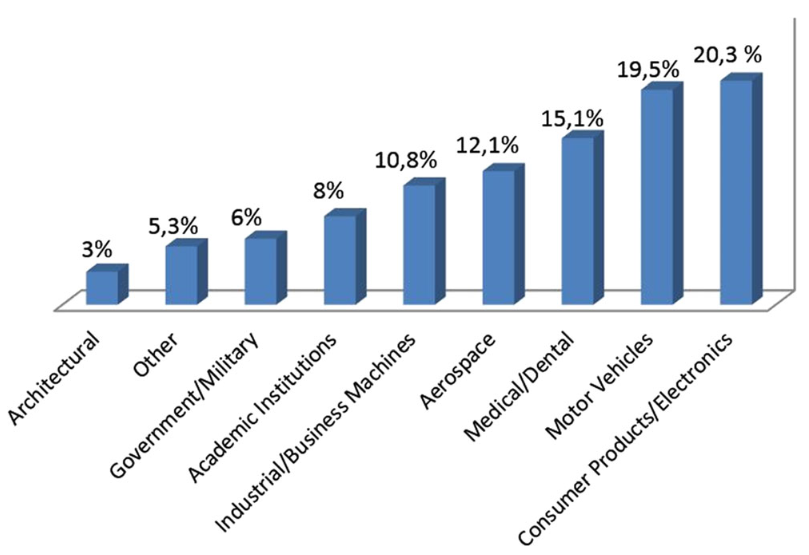
\includegraphics[scale=0.6]{bikas15industries}

    {\footnotesize Fonte: \citeauthor{bikas16}, \citeyear{bikas16}}
    \label{fig:MA_industrias}
    \end{center}
\end{figure}

\section{\textit{Fused Deposition Modeling}}
\textit{Fused Deposition Modeling} (FDM) ou \textit{Fused Filament Fabrication} 
(FFF) é uma das tecnologias MA mais populares como mencionado anteriormente.
Ela se consiste por depositar material através de um processo 
onde um filamento de material é forçado dentro de uma câmara através,
geralmente, de rolos dentados onde em uma região específica esse 
material é liquefeito. Por conta da pressão criada pelo filamento 
adentrando a câmara dentro do extrusor, ainda no estado sólido, 
o material liquefeito é extrudado através de um bocal, 
comumente fabricado de bronze. Então, o filamento liquefeito é 
depositado em uma plataforma de forma a percorrer a trajetória 
desejada utilizando mecanismos movidos de forma controlada, 
geralmente por motores de passos. O processo é repetido camada 
por camada, de forma que elas estejam apoiadas por camadas 
anteriores e a primeira camada continue fixa na plataforma ou 
cama, até que o processo finalize \cite{turner14}.
Podemos observar a disposição desses componentes na figura \ref{fig:fdm_ex}.

\begin{figure}[!htb]
    \begin{center}
    \caption{Principio e processo de impressão para FDM}
    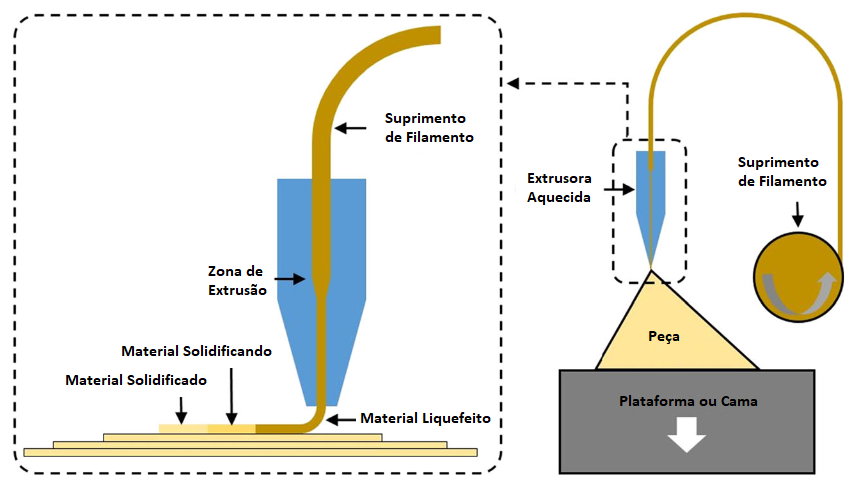
\includegraphics[scale=0.6]{bikas2015FDM}

    {\footnotesize Fonte:Adaptado de \citeauthor{bikas16}, \citeyear{bikas16}}
    \label{fig:fdm_ex}
    \end{center}
\end{figure}

O trabalho de \cite{vyavahare20} apresenta algumas 
características sobre o desenvolvimento científico sobre 
FDM ao longo dos anos, tendo como base 211 artigos diferentes 
de 1994 a 2020. É apresentado um grande salto no número de 
artigos publicados no tema em anos recentes (2015 a 2018) 
(figura \ref{fig:numero_artigos}), com 56\% dos temas trabalhados em torno da 
otimização de parâmetros de impressão, acompanhado de 17\% de 
trabalhos relacionados a aplicações utilizando o processo FDM, enquanto apenas 27\%
são relacionados ao restante dos temas, incluindo avanços tecnológicos relacionados
a melhorias de \textit{hardware} e \textit{software} desses dispositivos (\ref{fig:distr_artigos}).

\begin{figure}[!htb]
    \centering
    \caption{Número de aritos publicados sobre FDM ao longo do tempo}
    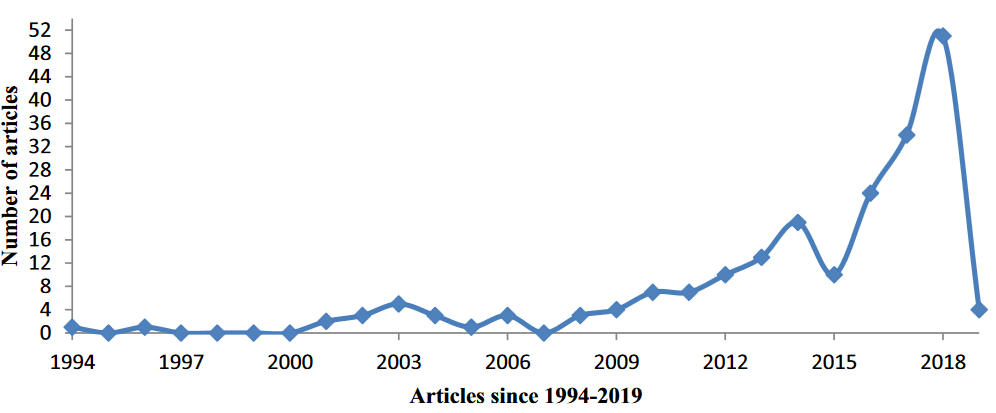
\includegraphics[scale=0.5]{vyan20npub}
    
    {\footnotesize Fonte: \citeauthor{vyavahare20}, \citeyear{vyavahare20}}
    \label{fig:numero_artigos}
\end{figure}

\begin{figure}[!htb]
    \centering
    \caption{Distribuição das pesquisas sobre FDM}
    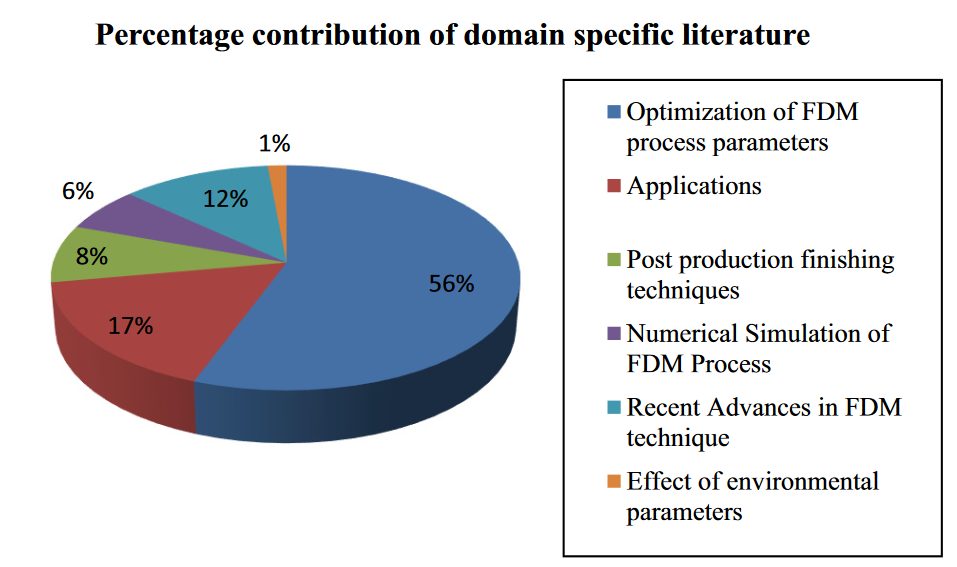
\includegraphics[scale=0.6]{vyan20oizzama}

    {\footnotesize Fonte: \citeauthor{vyavahare20}, \citeyear{vyavahare20}}
    \label{fig:distr_artigos}
\end{figure}


\section{Impressora 3d}

Extrusora: A extrusora é responsável por derreter o filamento de material termoplástico e extrudá-lo 
em forma de filamento derretido. 
Ela consiste em um bico aquecido (hotend) que funde o material e um motor que empurra o 
filamento através do bico. Alguns modelos mais avançados podem ter extrusoras duplas para 
imprimir com materiais diferentes ou suportes solúveis.

Mesa de impressão: A mesa de impressão é a superfície onde o objeto está sendo construído. 
Ela é aquecida em muitas impressoras FDM para ajudar a aderência do material à superfície. 
Além disso, algumas mesas de impressão têm características especiais, como superfícies 
texturizadas ou magnéticas, para facilitar a aderência e a remoção do objeto após a conclusão.

Plataforma de construção: A plataforma de construção é o suporte físico onde a mesa de impressão é montada. 
Ela pode ser ajustada em altura para nivelar a superfície de impressão e garantir que a primeira camada do 
objeto seja depositada com precisão.

Motor de movimento: Impressoras 3D FDM possuem motores de movimento que controlam a posição da extrusora e 
da mesa de impressão ao longo dos eixos X, Y e Z. Geralmente são motores de passo e seus movimentos de rotação
são geralmente convertidos em movimentos lineares através de correias ou parafusos de rosca trapezoidal.

Filamento: O filamento é o material de alimentação para a impressora 3D. Ele é um longo fio de plástico 
termoplástico que é inserido na extrusora e derretido durante o processo de impressão. Os filamentos vêm 
em várias cores e tipos de material, dependendo do objeto a ser impresso.

Software de fatiamento: Para imprimir um objeto em uma impressora 3D FDM, você precisa de um software de fatiamento. 
Este software converte modelos 3D em camadas finas onde é definido um percurso preenchendo essas camandas junto
a outros comandos e configurações, como a temperatura do bico injetor, as velocidades máximas desejadas de cada movimento,
a unidade utilizada, entre outras configurações e comandos. Estes comandos descritos através de Gcode e enviado para a impressora. 

Sistema de controle e geração de comando: A eletrônica de controle inclui a placa-mãe da impressora, que recebe comandos do 
software, em geral no formato Gcode, e os traduz em movimentos dos motores, controle de temperatura da extrusora e da mesa de impressão, 
velocidade dos ventiladores entre outros acessórios. 
Ela também pode ter uma tela de exibição e controles para operação manual.

Podemos separar, de maneira simplificada, o \textit{software} de impressoras 3D
FDM em três principais etapas: fatiamento (\textit{slicing}), geração de comando e controle.
A etapa de fatiamento envolve a topologia e a criação de instruções a partir do modelo digitalizado da peça a ser produzida,
é nessa fase onde se decide a sequência de movimentos e outros eventos.
Já na etapa de geração de comando, as instruções criadas pelo fatiador (\textit{slicer}) na etapa anterior
são interpretadas e os comandos detalhados são gerados, por exemplo as curvas de velocidade que ditarão a 
estratégia de trajetória para se realizar os diferentes deslocamentos na impressão.
Esses comandos são utilizados para movimentar os motores e outros equipamentos da impressora.
Na etapa de controle, uma etapa relativamente nova nas impressoras 3D mais acessíveis, 
técnicas de controle são utilizadas para se diminuir vibrações e variações indesejadas em quaisquer
parâmetros controlados, como a temperatura do bico. Um dos grandes avanços nessa etapa
foi a implementação da técnica de \textit{Input Shaping} por um \textit{firmware Open Source} de impressora 3D chamado Klipper,
que permitiu velocidades de impressão mais altas, sem a necessidade de alteração física de impressoras antigas \cite{klipperdoc}.


\subsection{Geração de comando}
A geração de comando é o processo que coordena a ativação dos 
atuadores, motores, dentre outros componentes de uma impressora. 
Ele recebe como base uma série de comandos que precisam ser 
interpretados e interpolados. Esse processo é responsável pelo 
controle de velocidade, aceleração dentre outras atividades que 
variam no tempo \cite{yu20}. 

\subsection{Gcode}

O G-code (Código G) é uma linguagem de programação usada em impressoras 3D e máquinas CNC para controlar o movimento e as ações da máquina durante o processo de fabricação. Ele é composto por uma série de comandos textuais, cada um com um formato específico. Aqui estão alguns elementos-chave da estrutura típica de um comando G-code:

\begin{itemize}
    \item Prefixo (Código G): Todo comando G-code começa com a letra 'G', que indica que é um comando de movimento ou função.
    \item Número do Comando: Após o 'G', segue um número que identifica o tipo específico de comando. Por exemplo, 'G0' é frequentemente usado para mover rapidamente a cabeça de impressão para uma posição, enquanto 'G1' é usado para movimentos de impressão lineares.
    \item Parâmetros: Após o número do comando, podem seguir-se parâmetros adicionais. Esses parâmetros variam dependendo do comando, mas podem incluir coordenadas de posicionamento (X, Y, Z), velocidades de movimento, taxas de alimentação, temperaturas e outros valores relevantes.
    \item Comentários: O G-code também pode incluir comentários precedidos por um ponto e vírgula (;) ou entre parênteses (). Os comentários não afetam a execução do programa, mas ajudam a documentar o código para facilitar a compreensão.
    \item Fim de Linha: Cada comando G-code é normalmente concluído com um caractere de fim de linha, como o retorno de carro ('\textbackslash n') ou a combinação de retorno de carro e nova linha ('\textbackslash r \textbackslash n'), dependendo do sistema.
\end{itemize}

\subsection{Curvas de velocidade trapezoidal}
As impressoras 3D entre outros equipamentos, como máquinas CNC, necessitam
de um planejamento de velocidade, pois o Gcode fornece apenas as velocidades máximas
de cada movimento, assim é necessário planejar o comportamento da velocidade ao longo tempo
dentro de cada comando.

Uma das maneiras mais simples para a criação dessa curva de velocidade é
de considerar as transições de velocidade com aceleração constante, criando 
um perfil de velocidade trapezoidal, em geral com 3 segmentos.
O primeiro segmento saindo da velocidade inicial para a velocidade máxima,
o segundo segmento com velocidade constante e o terceiro segmento saindo da velocidade máxima alcançada
para a velocidade final.
Em alguns casos as condições do comando e as configurações de aceleração não possibilitam que a impressora
alcance a velocidade máxima estabelecida no comando, nesses casos não existe o segundo segmento, ou seja, não existe
no perfil um estágio de velocidade constante.
\cite{yu20,klipperkinematic}.
(figura \ref{fig:trapezoidal}).

\subsection{\textit{Feedforward}}
Dentre os métodos de controle em aplicações FDM o \textit{Feedforward} 
é o mais eficiente dada as limitações de custo em impressoras 
3D comuns e é capaz de ter um impacto maior em sistemas 
conhecidos e sensíveis ao erro, onde buscam corrigir o erro 
antes que ele aconteça. As principais limitações da aplicação de técnicas \textit{Feedforward}
em impressoras 3D são a dificuldade de montar um modelo representativo,
a exigência computacional elevada e por fim a necessidade da simulação
se extender do incio ao fim, pela dependência de se basear no estado 
incial da impressão \cite{ramani20,duan18}.

\subsubsection{\textit{Input Shaper}}
Ao conhecer a trajetória desejada e as características do sistema, é possível calcular uma série de 
comandos que levam em consideração essas características para modificar o comando de referência. 
Isso permite que a trajetória final seja o mais próxima possível do comando de referência. 
Entretanto, ao invés de 
computar todo o comando de referência, é possível obter um 
comando modificado em tempo real através de um filtro. 
Uma das abordagens desse tipo de filtro de comando é o 
\textit{Input Shaper}, onde variados \textit{Shapers} são construídos levando 
em consideração diferentes objetivos e restrições 
\cite{singhose97}.
Podemos
ver na figura \ref{fig:degr_vs_esc} um exemplo comparativo
das respostas ao degrau e da função escada aplicada pelo \textit{shaper}.

\begin{figure}[!htb]
    \centering
    \caption{Comparação da resposta ao degrau e da resposta a escada}
    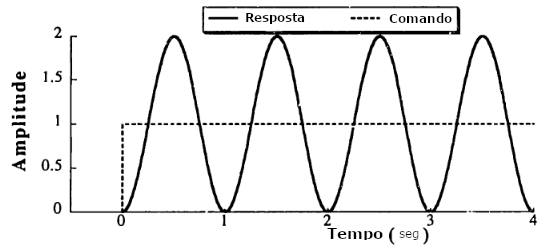
\includegraphics[scale=0.5]{inputshaperstepresponse1order}
    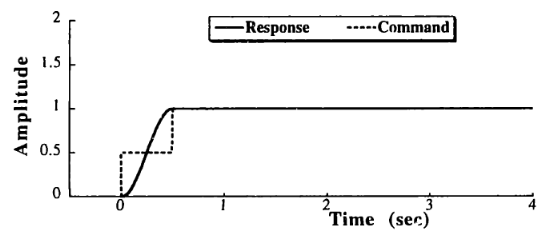
\includegraphics[scale=0.5]{inputshaperstarcasepresponse}

    {\footnotesize Fonte: \citeauthor{singhose97}, \citeyear{singhose97}}
    \label{fig:degr_vs_esc}
\end{figure}

Essa abordagem vem sendo explorada na comunidade "faça você mesmo" a partir de 2017 
quando a última patente desse método expirou, e tem aprimorado a área como
um todo, empurrando os limites anteriores de velocidade e precisão,
sendo popularizada pelo Klipper \cite{klipperkinematic}.

\subsubsection{\textit{Filtered basis function (FBF)}}
O método FBF necessita que a trajetória a ser rastreada seja totalmente
conhecida e que a trajetória controlada possa ser expressa como
uma combinação linear de funções base possuindo coeficientes desconhecidos.
As funções base são utilizadas em um controle \textit{feedforward} utilizando
o modelo dinâmico do sistema e selecionando os coeficientes de maneira a
minimizar os erros dada uma trajetória desejada (figura \ref{fig:flowchart_fbf}).
\cite{ramani17}

\begin{figure}[!htb]
    \centering
    \caption{Fluxograma FBF}
    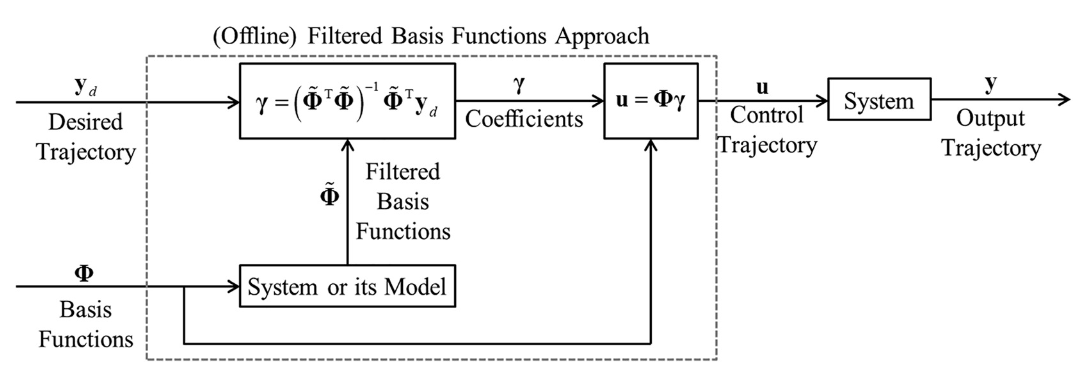
\includegraphics[scale=0.5]{ramani17blockfbf}

    {\footnotesize Fonte: \citeauthor{ramani17}, \citeyear{ramani17}}
    \label{fig:flowchart_fbf}
\end{figure}

Uma das maiores dificuldades que os métodos avançados para o
controle \textit{feedforward} de trajetórias é a necesidade de se conhecer
completamente a trajetória desejada, o que implica em um grande custo
computacional, principalmente em situações onde são necessárias uma
grande quantidade de amostras da trajetória, por exemplo em casos de alta resolução
e casos de longa duração.
O \textit{limited-preview filtered B-splines} adapta a solução do FBF de forma a dividir a 
trajetória desejada em subgrupos com um número menor de amostras e utiliza um algorítmo de 
\textit{receiding horizon} para calcular recursivamente os coeficientes da função B-spline que 
minimizam os erros de trajetória \cite{duan18}.

A partir dessa otimização da divisão da trajetória em subgrupos, esse método
conseguiu ser testado utilizando uma impressora 3D de verdade com modelos simples.
Apresentando resultados promissores apresentados na figura \ref{fig:duancubo}.

\begin{figure}[!htb]
    \centering
    \caption{Resultados práticos da LPFBF}
    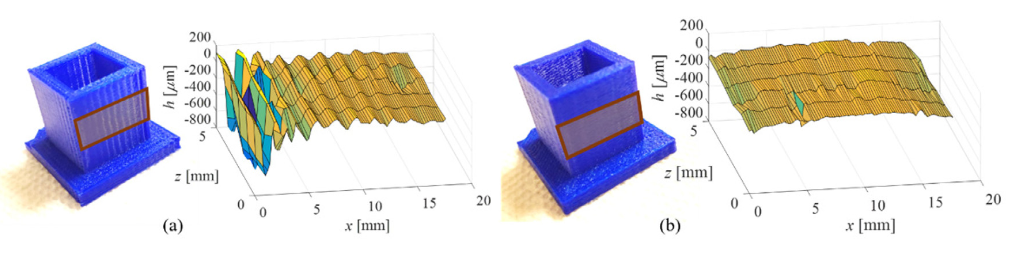
\includegraphics[scale=0.5]{duancubo}

    {\footnotesize Fonte: \citeauthor{duan18}, \citeyear{duan18}}
    \label{fig:duancubo}
\end{figure}

Com base nos desenvolvimentos nos trabalhos de \cite{ramani17} e \cite{duan18}, comentados anteriormente, 
\cite{ramani20} busca atacar um segundo desafio pratico na implementação da FBF, sendo o primeiro desafio prático
o custo computacional que foi endereçado pelo trabalho de \cite{duan18} através da LBFBF, permitindo a aplicação
do algoritmo no mundo real.

Este segundo desafio se trata da degradação de precisão de rastreamento da abordagem FBF, causada por
imprecisões no modelo ou incertezas na dinâmica da planta atrelado a característica do método de se
utilizar puramente uma abordagem de \textit{feedforward}. A não participação de \textit{feedbacks} sensoriais
do mundo real abre espaço para uma crescente divergência entre o modelo e a realidade.

Considerando o requisito de manter a performance computacional alcançada com o método LPFBF, \cite{ramani20} 
propõe, também, a utilização de um filtro robusto em substituição à dinâmica nominal da planta para 
filtrar as funções de base. Esse filtro robusto é construído com base no inverso de um controlador 
feedforward ótimo, que minimiza uma função de custo de erro para lidar com a incerteza conhecida da planta 
como um filtro robusto.
O esquema do método é apresentado na figura \ref{fig:flowchart_rfbf}.

\begin{figure}[!htb]
    \centering
    \caption{Fluxograma RFBF}
    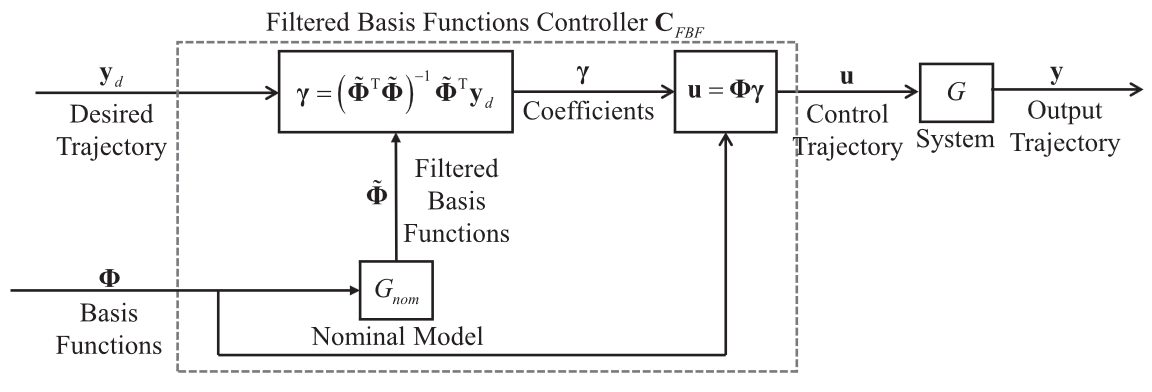
\includegraphics[scale=0.5]{ramani20blockfbf}

    {\footnotesize Fonte: \citeauthor{ramani20}, \citeyear{ramani20}}
    \label{fig:flowchart_rfbf}
\end{figure}

\section{Sistema massa mola}

\section{Espaço de Estados}

Os sistemas dinâmicos podem ser descritos através de uma formulação
chamada de espaço de estados, que tem como objetivo expressar modelos 
de equações diferencias parciais (EDP) ou ordinárias (EDO) de ordem superior
como um conjunto de EDPs ou EDOs de primeira ordem.
Essa formulação é construida a partir de um principio de autoregressão
das equações. Na equação \ref{eq:edo_ex} podemos observar uma EDO de segunda ordem representando
um sistema massa mola simples,
logo abaixo (\ref{eq:espaco_de_estados_ex}) a mesmsa equação representada na formulação
de espaço de estados \cite{hamilton94}.

\begin{equation}
    \label{eq:edo_ex}
    m \ddot x+c \dot x+kx = f(t)
\end{equation}

\begin{equation}
    \label{eq:espaco_de_estados_ex}
    \begin{bmatrix}
        \dot x \\
        \ddot x
    \end{bmatrix}
    =
    \begin{bmatrix}
        0 & 1 \\
        k/m & c/m
    \end{bmatrix}
    \begin{bmatrix}
        x \\
        \dot x
    \end{bmatrix}
    +
    \begin{bmatrix}
        0 \\
        1
    \end{bmatrix}
    f(t)
\end{equation}

\section{Integração implicita utilizando programação não linear}

\citeauthor{hargraves87} (\citeyear{hargraves87}) descreve um algoritmo para a solução numérica direta de problemas de controle ótimo. 
Este algorítmo emprega uma abordagem que utiliza polinômios cúbicos para representar as variáveis de estado. Adicionalmente, recorre à interpolação linear para tratar as variáveis de controle. 
Esse enfoque converte efetivamente o problema de controle ótimo em um problema de programação matemática.

Uma das principais vantagens desse método é sua facilidade de implementação e sua capacidade de lidar com uma ampla gama de problemas de otimização de trajetória. Isso inclui a consideração de restrições de caminho, estados descontínuos e desigualdades de controle.

O método alcança sua aproximação das soluções das equações diferenciais através da subdivisão de cada estado na matriz de espaço de estados em segmentos. Cada um desses segmentos é representado por polinômios de terceiro grau.

Os valores de estado são então selecionados de maneira a garantir que a curva resultante da concatenação desses polinômios seja continua, ou seja,
o valor da função e de sua derivada precisa ser igual para ambos polinômios nas conexões como observado na figura \ref{fig:hargraves_fun}

\begin{figure}[!htb]
    \centering
    \caption{Ilustração integração implícita}
    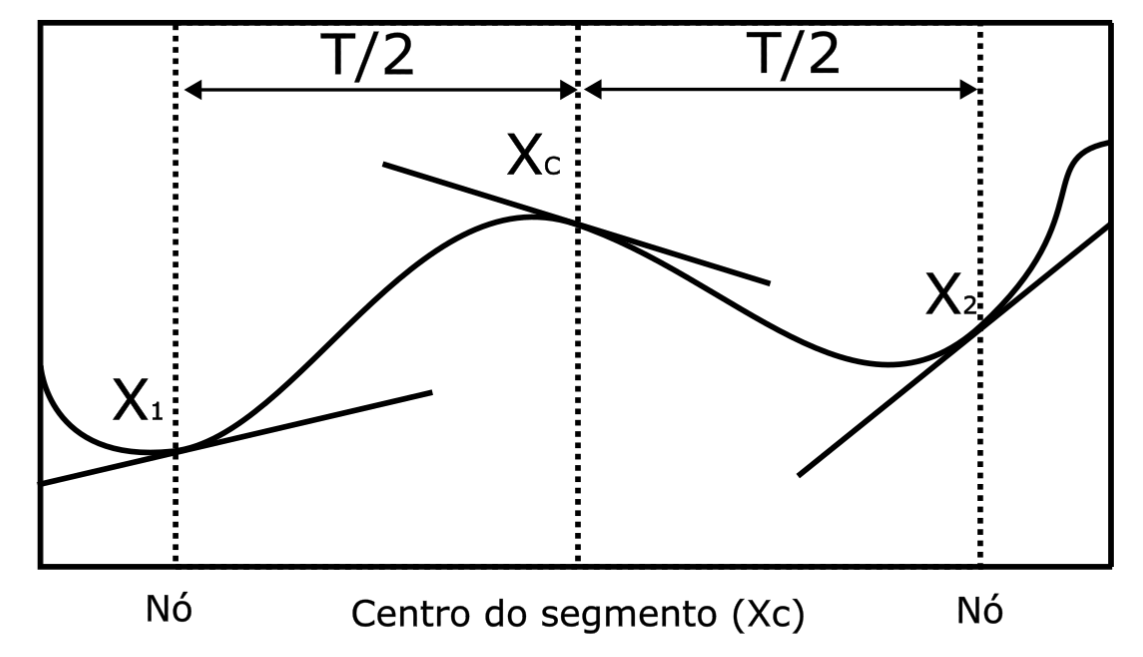
\includegraphics[scale=0.5]{hargraves_func}

    {\footnotesize Fonte: \citeauthor{hargraves87}, \citeyear{hargraves87}}
    \label{fig:hargraves_fun}
\end{figure}

O procedimento base pode ser aplicado pelos seguintes passos.

A equação \ref{eq:state_center_segment} avalia o estado no centro do segmento, onde $x$ representa o estado, 
T representa o comprimento do segmento e $f_i$ representa o valor da função avaliado em $x_i$.
O subscrito c representa o centro do segmento.

\begin{equation}
    \label{eq:state_center_segment}
    x_c = \frac{x_{1} + x_{2}}{2} + T\frac{f_{1} - f_{2}}{8}
\end{equation}

Da mesma maneira sua derivada é apresentada na equalção \ref{eq:state_dot_center_segment}.

\begin{equation}
    \label{eq:state_dot_center_segment}
    \dot{x_{c}} = -3\frac{x_{1} + x_{2}}{2T} + \frac{f_{1} + f_{2}}{4}
\end{equation}

A equação \ref{eq:defect_calc} define então o valor do defeito no centro do segmento.

\begin{equation}
    \label{eq:defect_calc}
    \Delta = f_c - \dot{x_c}
\end{equation}

Considerando também que a entrada do sistema pode ser avaliada de forma aproximada no centro do segmento 
através da equação \ref{eq:input_value_center_segment}.

\begin{equation}
    \label{eq:input_value_center_segment}
    u_c = \frac{u_1 + u_2}{2}
\end{equation}

Os valores de estado agora podem ser alterados de maneira que o defeito tenda a zero.

